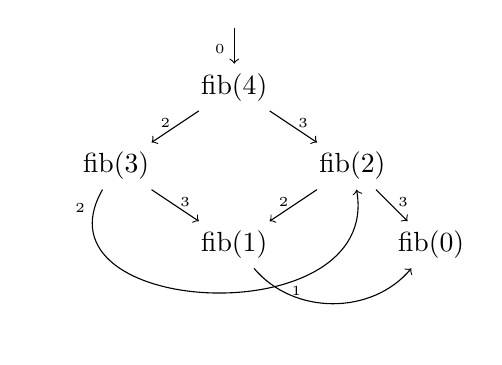
\begin{tikzpicture}
% nodes
\node (f4)     at (2.5, 2) {fib(4)};
    \node (f3) at (1, 1) {fib(3)};
        \node (f1) at (2.5, 0) {fib(1)};
    \node (f2) at (4, 1) {fib(2)};
        \node (f0) at (5, 0) {fib(0)};
% arrows
\draw[<-] (f4) -- node[pos=0.4, left, label distance=5mm]{\tiny{0}} +(0, 0.75);

\draw[->] (f4) -- node[pos=0.4, left, label distance=5mm]{\tiny{2}} (f3);
\draw[->] (f4) -- node[pos=0.4, right, label distance=5mm]{\tiny{3}} (f2);

    \draw[->, bend right=100, out=240, looseness=1.5] (f3) to node[pos=0.05, left, label distance=5mm]{\tiny{2}} (f2);
    \draw[->] (f3) -- node[pos=0.4, right, label distance=5mm]{\tiny{3}} (f1);
    \draw[->] (f2) -- node[pos=0.4, left, label distance=5mm]{\tiny{2}} (f1);
        \draw[->, bend right=50] (f1) to node[pos=0.2, right, label distance=5mm]{\tiny{1}} (f0);
    \draw[->] (f2) -- node[pos=0.4, right, label distance=5mm]{\tiny{3}} (f0);
\end{tikzpicture}